\subsection{Results}

In this study, participants had an average of 3.3 target sites enabled. They visited at least one target site 64\% of days on average. On each of those days, participants experienced interventions an average of 6.8 times.

%\subsection{RQ3 (revisited): Does randomizing which interventions are shown each visit have any effects on attrition, compared to always showing the same one?}

\begin{figure}
\centering
	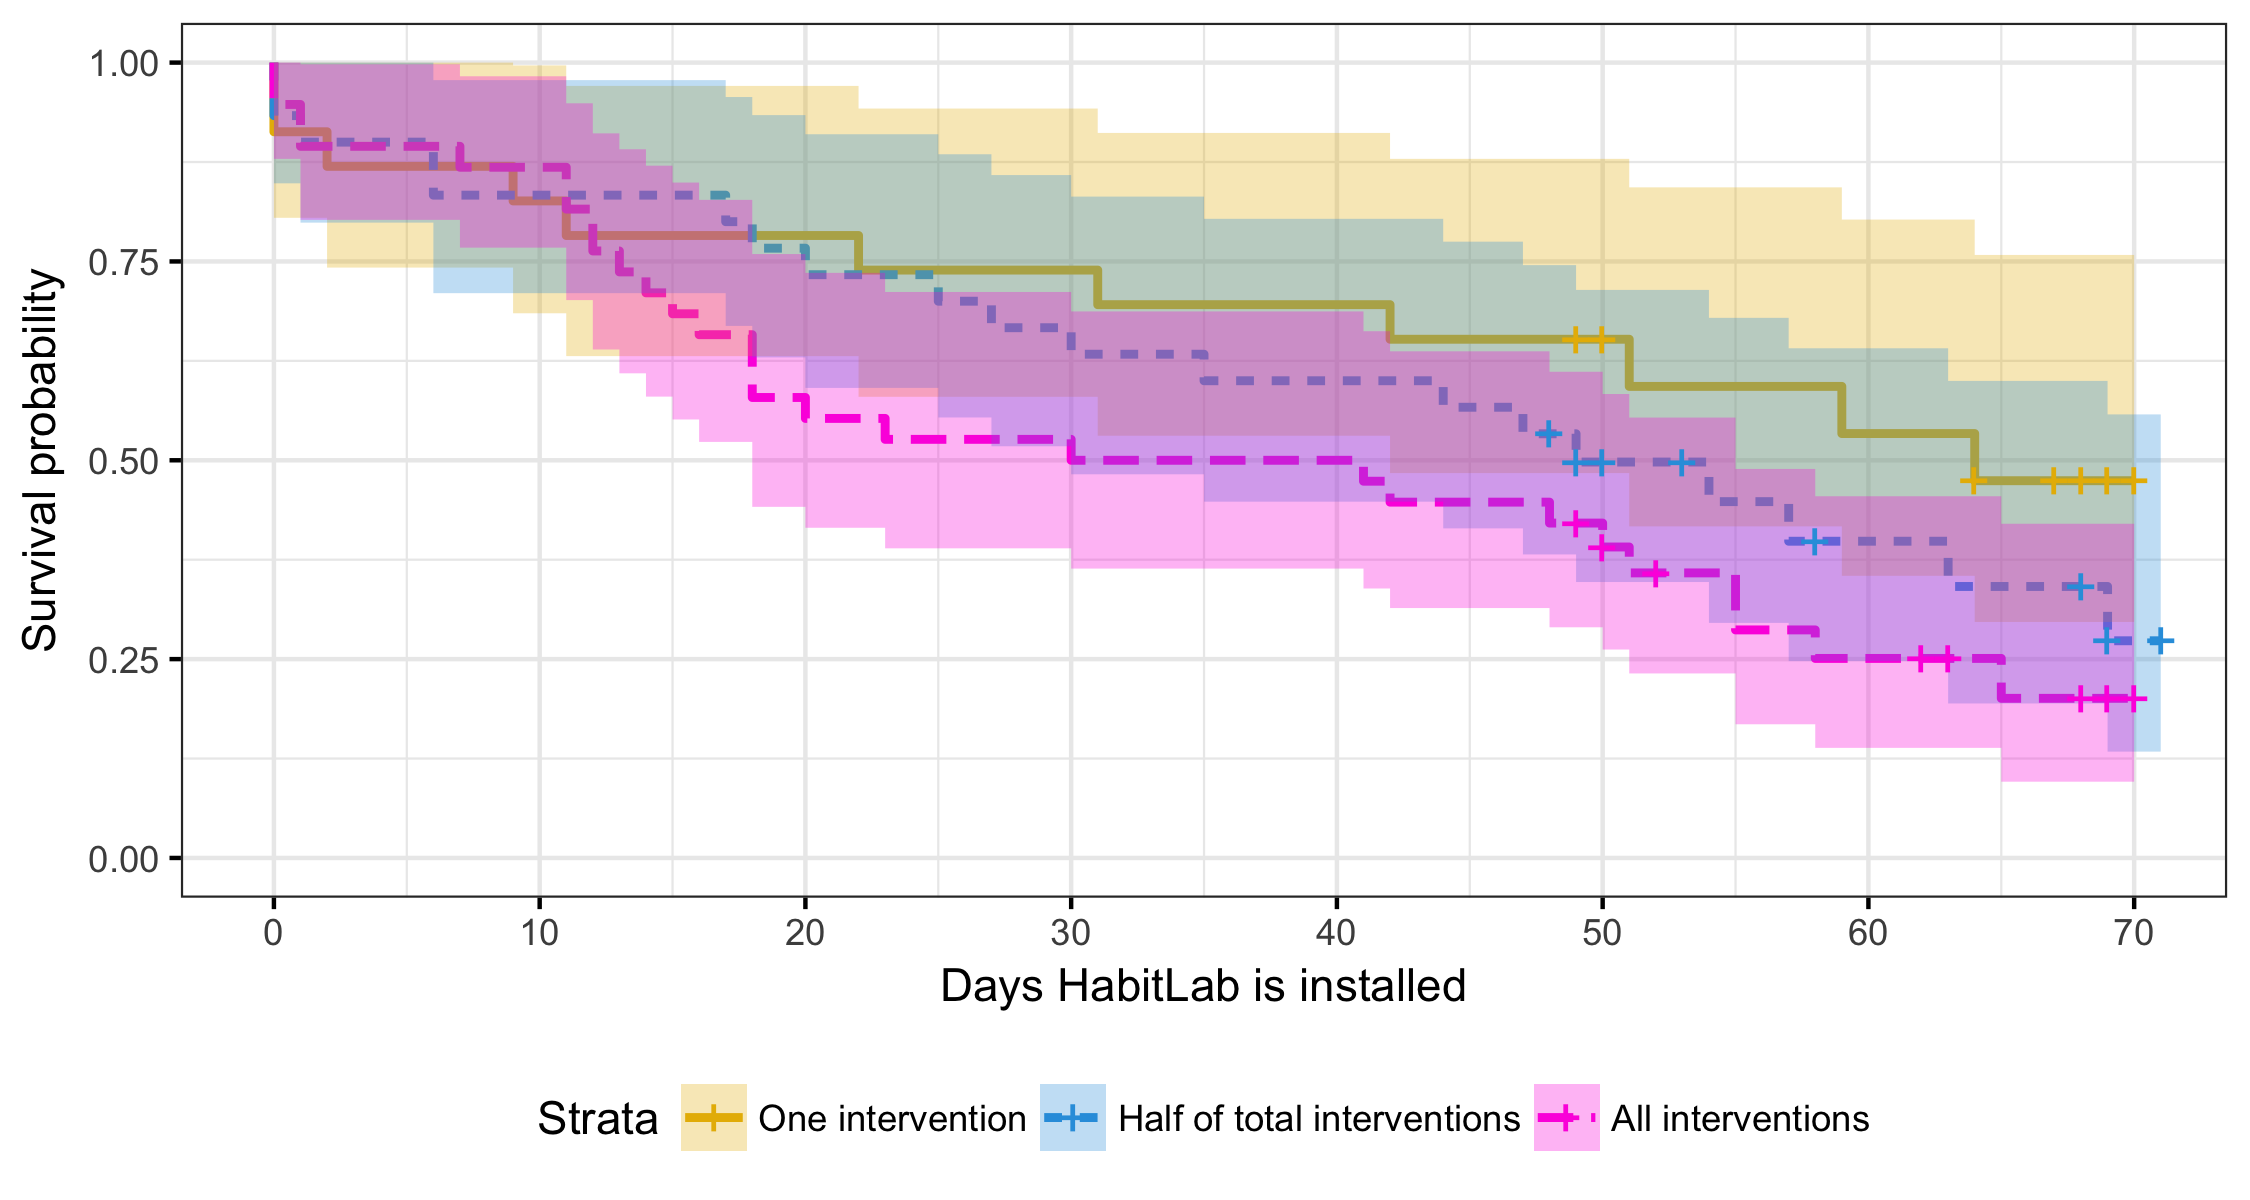
\includegraphics[width=1.0\textwidth]{figures/attrition_between_subjects.png}
	\caption{Including all interventions resulted in significantly more attrition than just one intervention.}
\label{fig:attrition_between_subjects}
\end{figure}

% Table created by stargazer v.5.2 by Marek Hlavac, Harvard University. E-mail: hlavac at fas.harvard.edu
% Date and time: Thu, Apr 19, 2018 - 09:01:42
\begin{table}[tb] \centering 
  \caption{A Cox proportional hazards analysis over a longer period suggests that rotating with more interventions increases the hazard of attrition.} 
  \label{tab:cox_regression_between_participants} 
\begin{tabular}{@{\extracolsep{5pt}}lc} 
\\[-1.8ex]\hline 
\hline \\[-1.8ex] 
 & \multicolumn{1}{c}{\textit{Dependent variable:}} \\ 
\cline{2-2} 
\\[-1.8ex] & Log hazard ratio \\ 
\hline \\[-1.8ex] 
 Half of total interventions (baseline: one intervention) & 0.395 \\ 
  & (0.380) \\ 
  All interventions & 0.711$^{*}$ \\ 
  & (0.358) \\ 
 \hline \\[-1.8ex] 
Observations & 91 \\ 
\hline 
\hline \\[-1.8ex] 
\textit{Note:}  & \multicolumn{1}{r}{$^{*}$p$<$0.05; $^{**}$p$<$0.01; $^{***}$p$<$0.001} \\ 
\end{tabular} 
\end{table} 

% (this is from the between-subjects study)

%We restricted our analysis to users who kept the default interventions during the first 5 minutes -- the same result can be obtained if we restrict our analysis to users who kept the default interventions during the entire period. Thus, the ``all defaults'' condition becomes equivalent to the ``rotation'' condition from Study 1, and the ``one default'' condition becomes equivalent to the ``static'' condition from Study 1.

In this longer, between-subjects experiment, attrition rates were significantly higher in the all interventions condition (Figure~\ref{fig:attrition_between_subjects}, Table~\ref{tab:cox_regression_between_participants}). This agrees with the analogous result from Study 1 showing a higher attrition rate for the rotation condition. The half of total interventions survival curve falls in between that of the one intervention and all interventions conditions, but does not have a statistically significant difference.

% \rev{What is the range of attrition rates between conditions? We can estimate a lower bound on attrition rate by looking at the subgroup with the lowest attrition. The group with the lowest attrition in the single intervention condition of this study were users in the one intervention condition whose only intervention was X. This had a retention rate of N\% over the course of M weeks.}

\begin{comment}
\subsection{RQ4: Are users who enable or disable interventions during onboarding less likely to attrition?}

%(this is actually from the between-subjects study)

\begin{figure}
\centering
	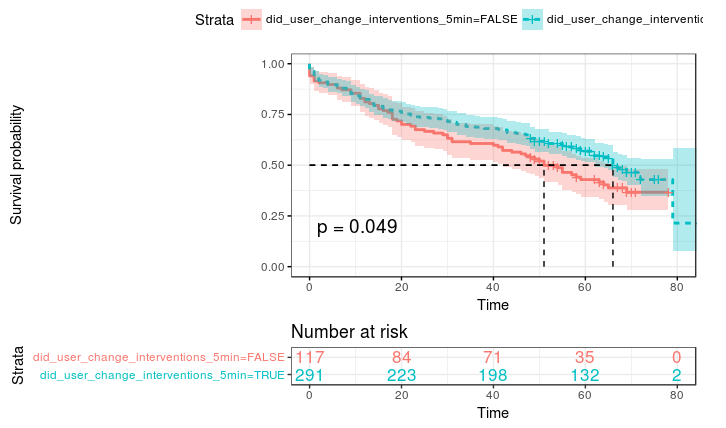
\includegraphics[width=1.0\textwidth]{figures/attrition_between_changed_interventions.png}
	\caption{Users who change interventions during the first 5 minutes will be significantly less likely to attrition later.}
\label{fig:attrition_between_changed_interventions}
\end{figure}

We compared users who enabled or disabled interventions during the first 5 minutes, compared to other users who completed the onboarding process without enabling or disabling any interventions. We found that users who enabled or disabled interventions during the first 5 minutes had a significantly lower rate of attrition, as shown in Figure~\ref{fig:attrition_between_changed_interventions}.



% \msb{TODO: what can we not generalize, given the design of our experiment and measures?}

\end{comment}